
\documentclass[letterpaper,12pt]{article}
\usepackage{tabularx} % extra features for tabular environment
\usepackage{amsmath}  % improve math presentation
\usepackage{float}
\usepackage{pdfpages}

\usepackage{multicol}
\usepackage{graphicx} % takes care of graphic including machinery
\graphicspath{ {./figures/} }
%\usepackage[margin=1in,letterpaper]{geometry} % decreases margins
%\usepackage{cite} % takes care of citations
\usepackage[final]{hyperref} % adds hyper links inside the generated pdf file
\hypersetup{
	colorlinks=true,       % false: boxed links; true: colored links
	linkcolor=blue,        % color of internal links
	citecolor=blue,        % color of links to bibliography
	filecolor=magenta,     % color of file links
	urlcolor =blue         
}
\usepackage[margin = 1in,headsep=0.5cm,headheight=2cm,letterpaper]{geometry} 

\usepackage{fancyhdr}
\pagestyle{fancy}
\lhead{Student 1 : Ahmet Akman 2442366 \\ Student 2: Yusuf Toprak Yıldıran 2444149 \\ Assistant: Onur Selim Kılıç}
\rhead{Date: \today \\ Group: Wednesday Morning - 5} 
%\cfoot{center of the footer!}
\renewcommand{\headrulewidth}{0.1pt}



\begin{document}
\thispagestyle{empty}

\title{Spring 2022 EE214 Experiment 6  \protect\\ Frequency Response}
\author{Ahmet Akman 2442366 \protect\\ Yusuf Toprak Yıldıran 2444149 \protect\\ Assistant: Onur Selim Kılıç}
\date{\today}
\maketitle
\tableofcontents
%\begin{abstract}
%abstract
%\end{abstract}
\section{Introduction}
In this experiment, Frequency Response, four different setups of filter circuits will be experimented with. First, a high pass filter with a resistor and a capacitor will be set, and its characteristics will be observed. Then a lowpass filter with an inductor and a resistor will be constructed, and its behavior will be observed. A high-q RLC bandpass filter will be set, and its quality factor will be determined. Lastly, a square wave is applied to the bandpass, and a half rectified sinusoidal is filtered. As a result, the waves that are included in a signal need to be observed.
\section{Experimental Results and Discussion}
The results of the experiment are discussed in the following steps.

\subsection{Step 1}
In this step, circuit given in Figure 1 is set with its settings and sine wave of 10V peak is adjusted.
\begin{figure}[H]
    \centering
    \includegraphics[width = 0.75\textwidth]{{highpass.png}}
    \caption{Circuit schematic for step 1}
\end{figure} 
\subsubsection{a.}
For this part, half-power angular frequency is determined by changing the input frequency manually until observing \(V_0\) equals 0.7 times of input voltage, and the cutoff frequency(half-power frequency) is found as approximately 500Hz.
\subsubsection{b.}
For this part, magnitude and phase responses of the circuit in Figure 1 are obtained by using the BenchVue test flow. In order to do this,
\begin{itemize}
    \item Agilent Signal Generator and oscilloscope are intialized with 20V pp.
    \item Test flow is constructed by using sweep option from \(\frac{f_c}{5}\)(half-power frequency/5) to \(5f_c\) with \(\frac{f_c}{5}\) steps.
    \item After running the test, magnitude vs frequeny plot is obtained. 
    \item Then, data is imported to MATLAB and magnitude and phase response plots are obtained by indicating the cutoff frequency in te plot.
\end{itemize}
To obtain magnitude ch2 voltage measurement vector is divided by the ch1 voltage measurement vector pairwise(using ./), and magnitude response is plotted as magnitude on the y axis, and frequency measurement is on the x-axis in Figure 2.
\begin{figure}[H]
    \centering
    \includegraphics[width = 0.75\textwidth]{{1_1_1.png}}
    \caption{Magnitude response of circuit 1}
\end{figure} 
To obtain phase response, a plot in which mod(phase-measurement+180,360)-180 is on the y axis and the frequency measurement vector is on the x-axis is obtained in Figure 3.
\begin{figure}[H]
    \centering
    \includegraphics[width = 0.75\textwidth]{{1_1_2.png}}
    \caption{Frequency response of circuit 1}
\end{figure} 
Since high pass filter allows frequencies that greater than the cutoff frequency to pass, by looking at the magnitude response it can be said that this filter is highpass filter.

\subsection{Step 2}
In this step the circuit given in Figure 4 is constructed. The switch was kept open. 
\begin{figure}[H]
    \centering
    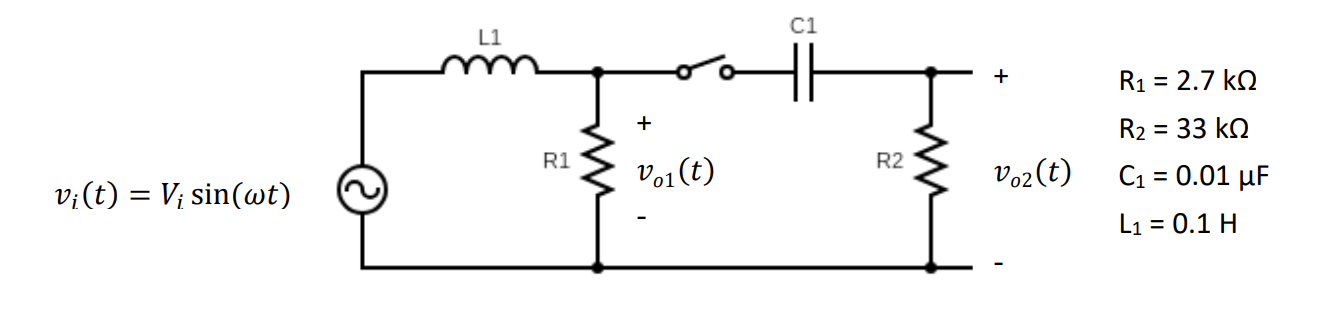
\includegraphics[width = 0.75\textwidth]{lowqlowpass.png}
    \caption{Circuit schematic for the step 2}
\end{figure} 
Then similar to the previous step, a test flow on the BenchVue is run. Then the outputs of the test flow are exported as a MATLAB data file. The data is imported in MATLAB. The plots of phase response and magnitude response are plotted, which are given in Figures 5 and 6.
\begin{figure}[H]
    \centering
    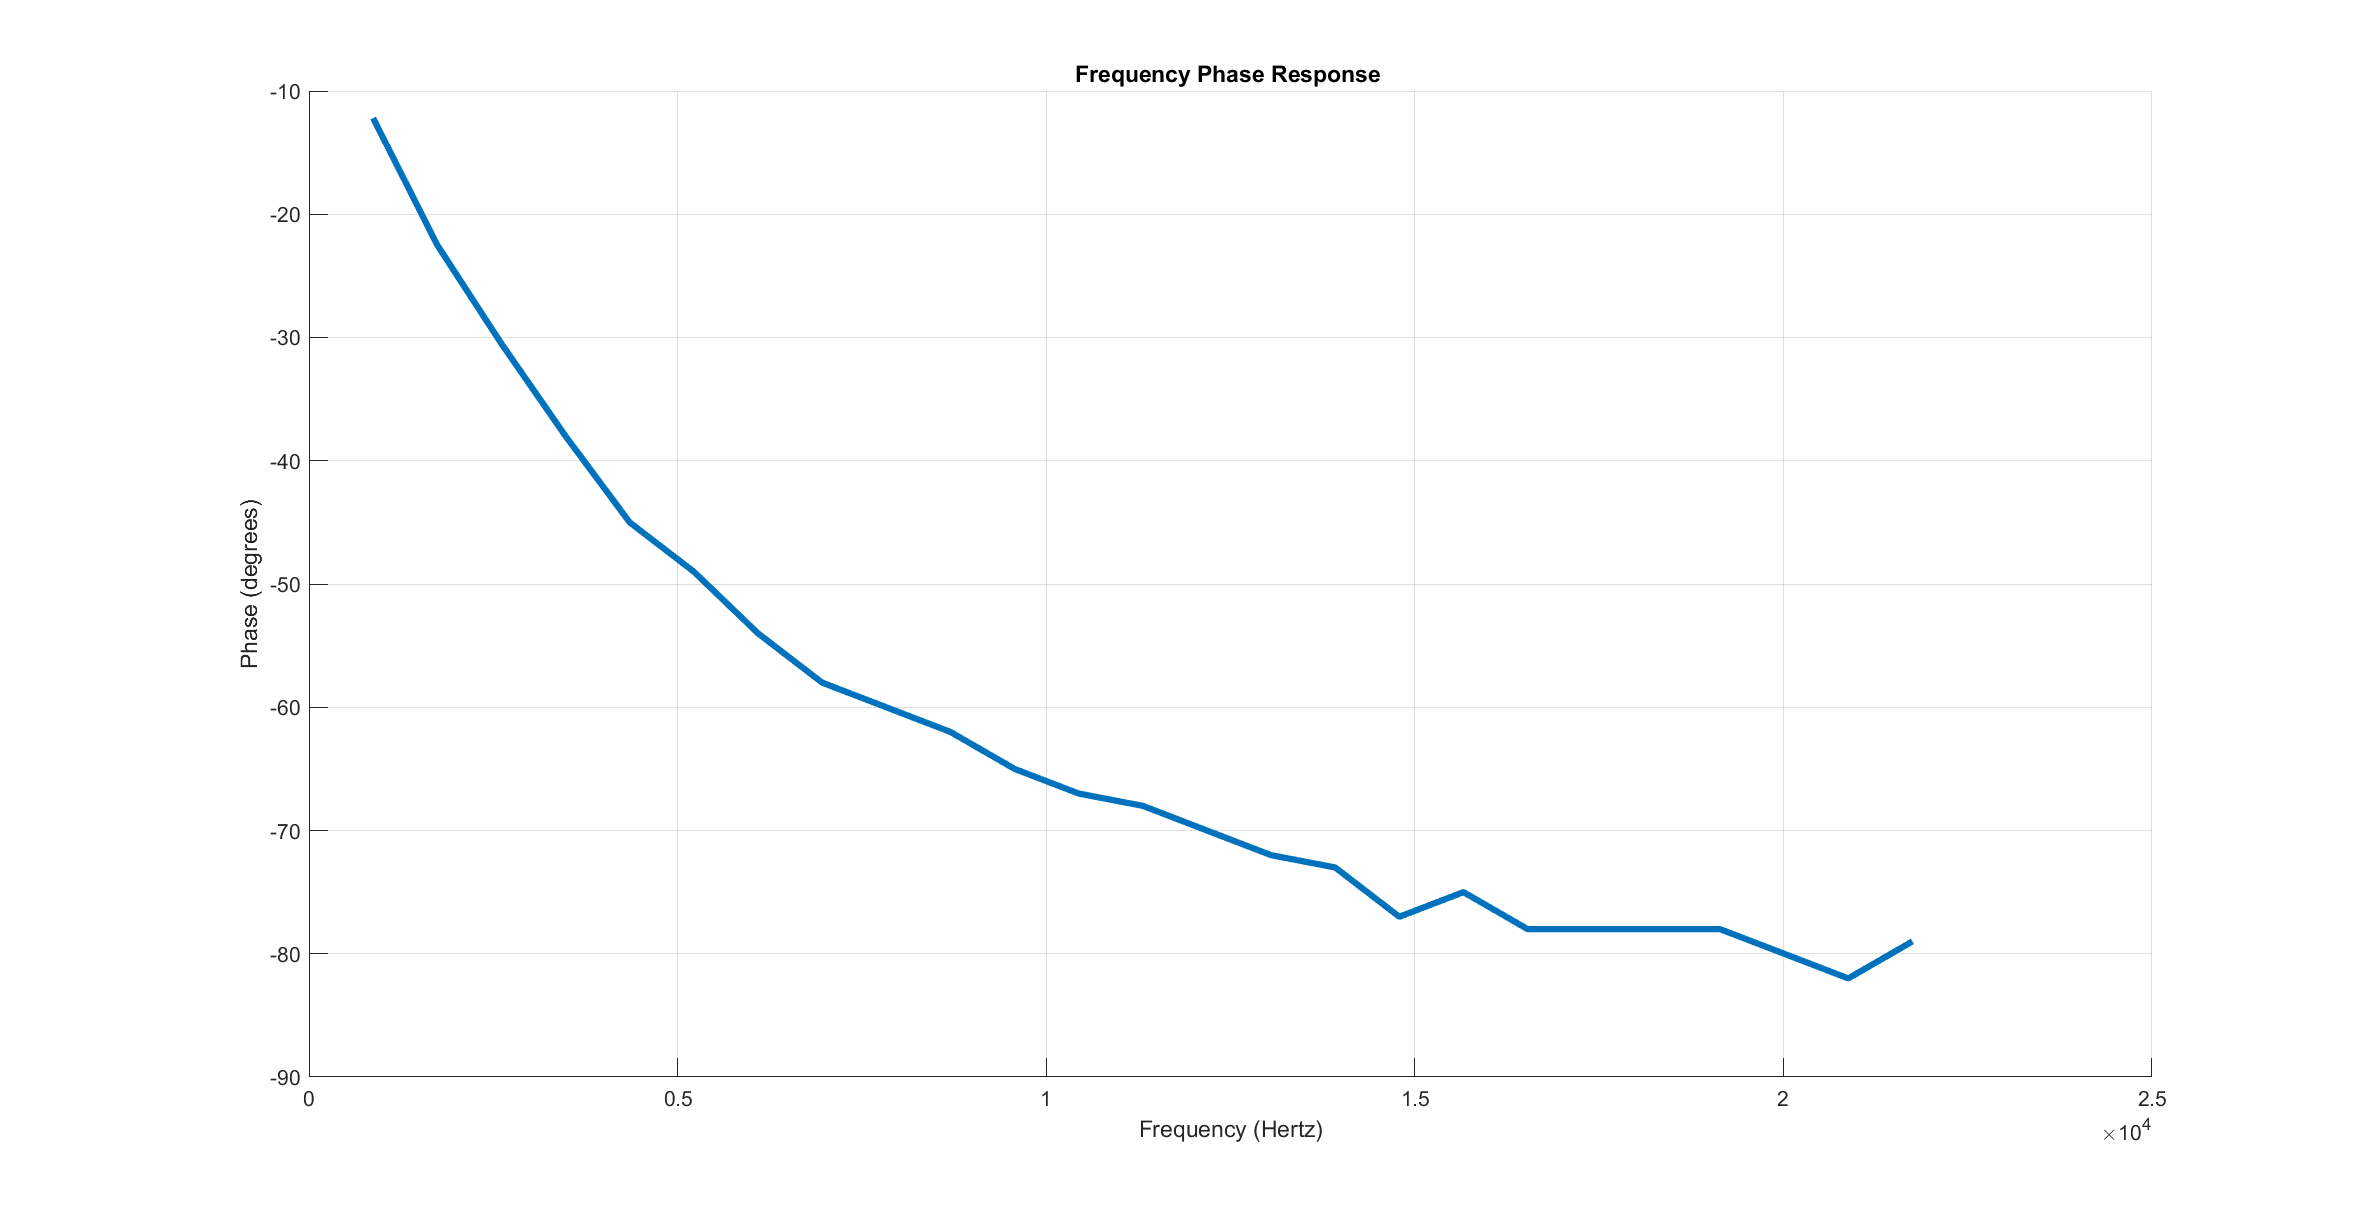
\includegraphics[width = 0.75\textwidth]{2_1_2.png}
    \caption{Phase Response of the Low-Q RL filter.}
\end{figure} 

\begin{figure}[H]
    \centering
    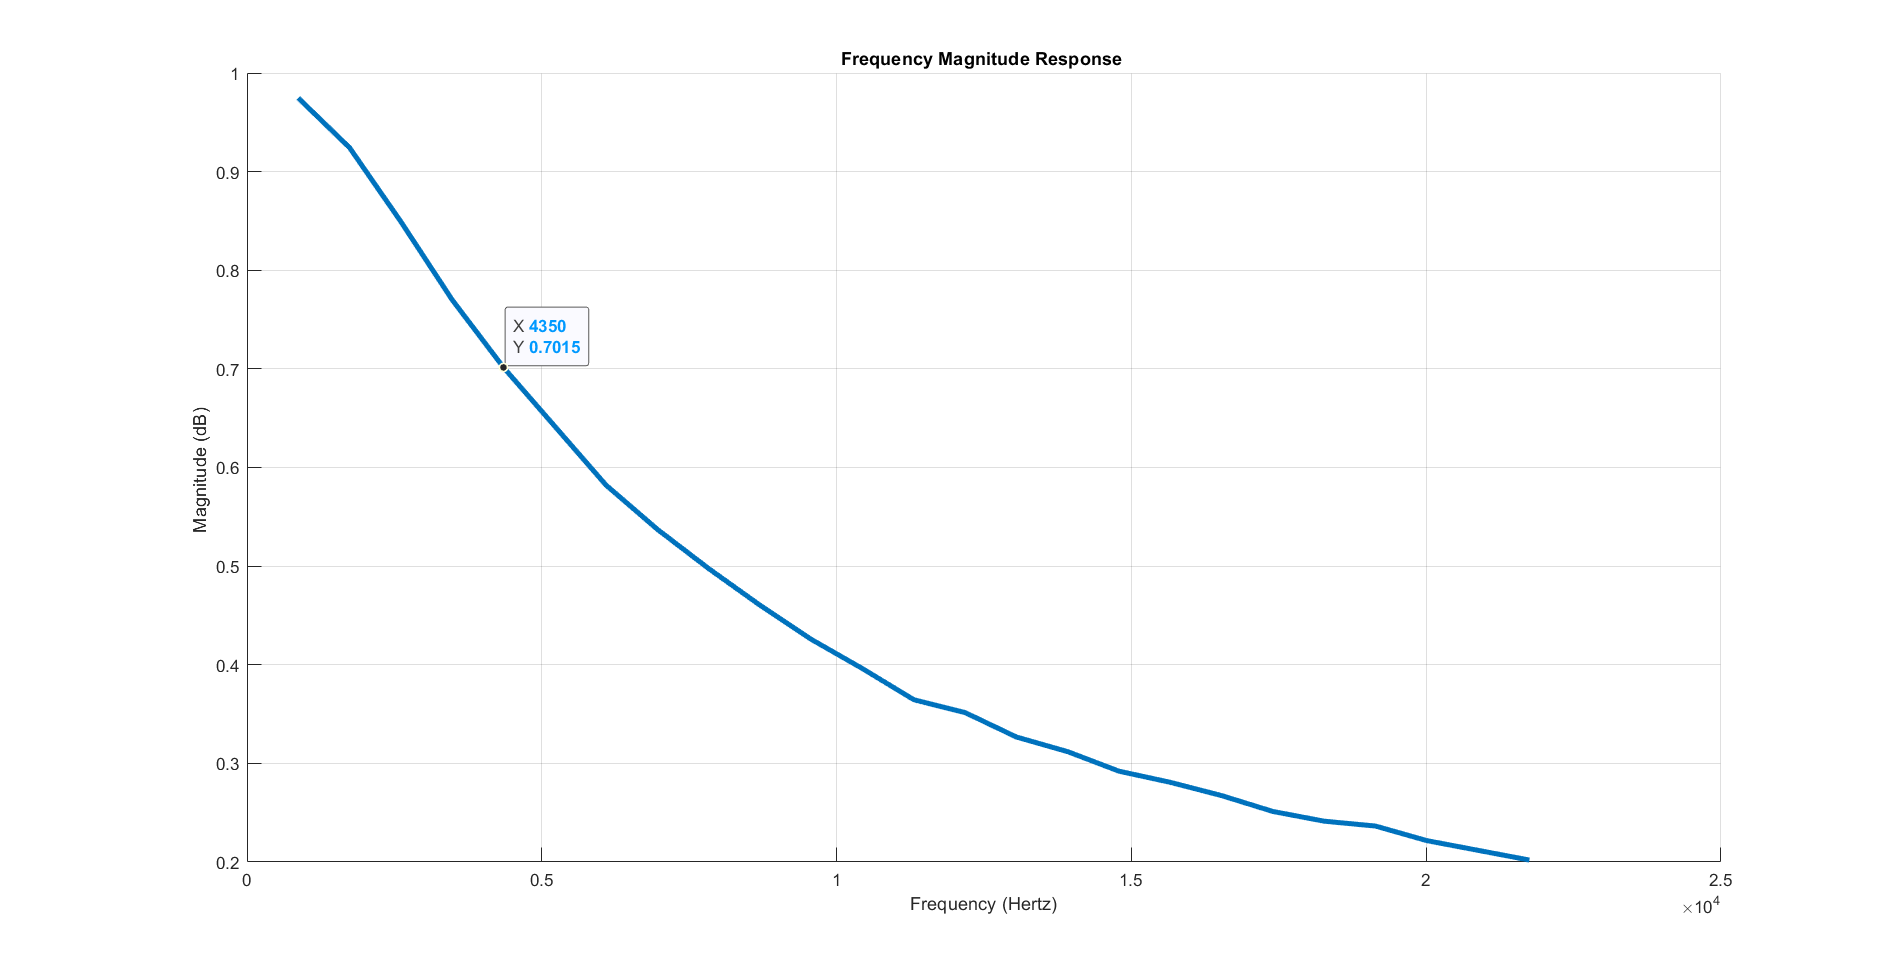
\includegraphics[width = 0.75\textwidth]{2_1_1.png}
    \caption{Magnitude Response of the Low-Q RL filter.}
\end{figure} 
The value of the \(\omega_c\) is pinned in the magnitude response plot. As a result, it can be concluded that the circuit is an example of a passive low pass filter. Low pass filters allow only the frequencies below the threshold. By looking at the sharpness of the responses, it can be said that the Q (the quality factor) of the circuit is low. 
    
\subsection{Step 3}
In this step the circuit given in Figure 7 is set on the breadboard. The C value is taken as 0.01\(\mu F\) as it was found in the preliminary work. 
\begin{figure}[H]
    \centering
    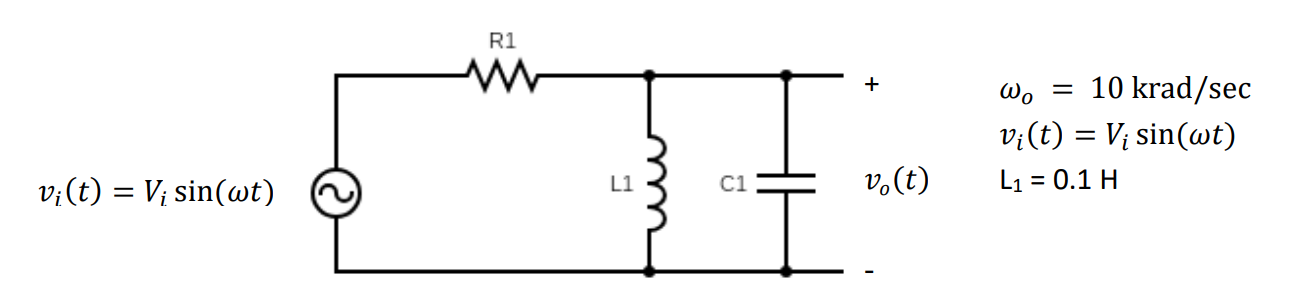
\includegraphics[width = 0.75\textwidth]{highqbandpass.png}
    \caption{Circuit schematic for the step 3}
\end{figure} 
Then similar to the previous steps, the test flow on BenchVue is run. The results are exported to a Matlab data file. The data is imported in MATLAB. The plots of phase response and magnitude response are plotted, which are given in Figures 8 and 9.
\begin{figure}[H]
    \centering
    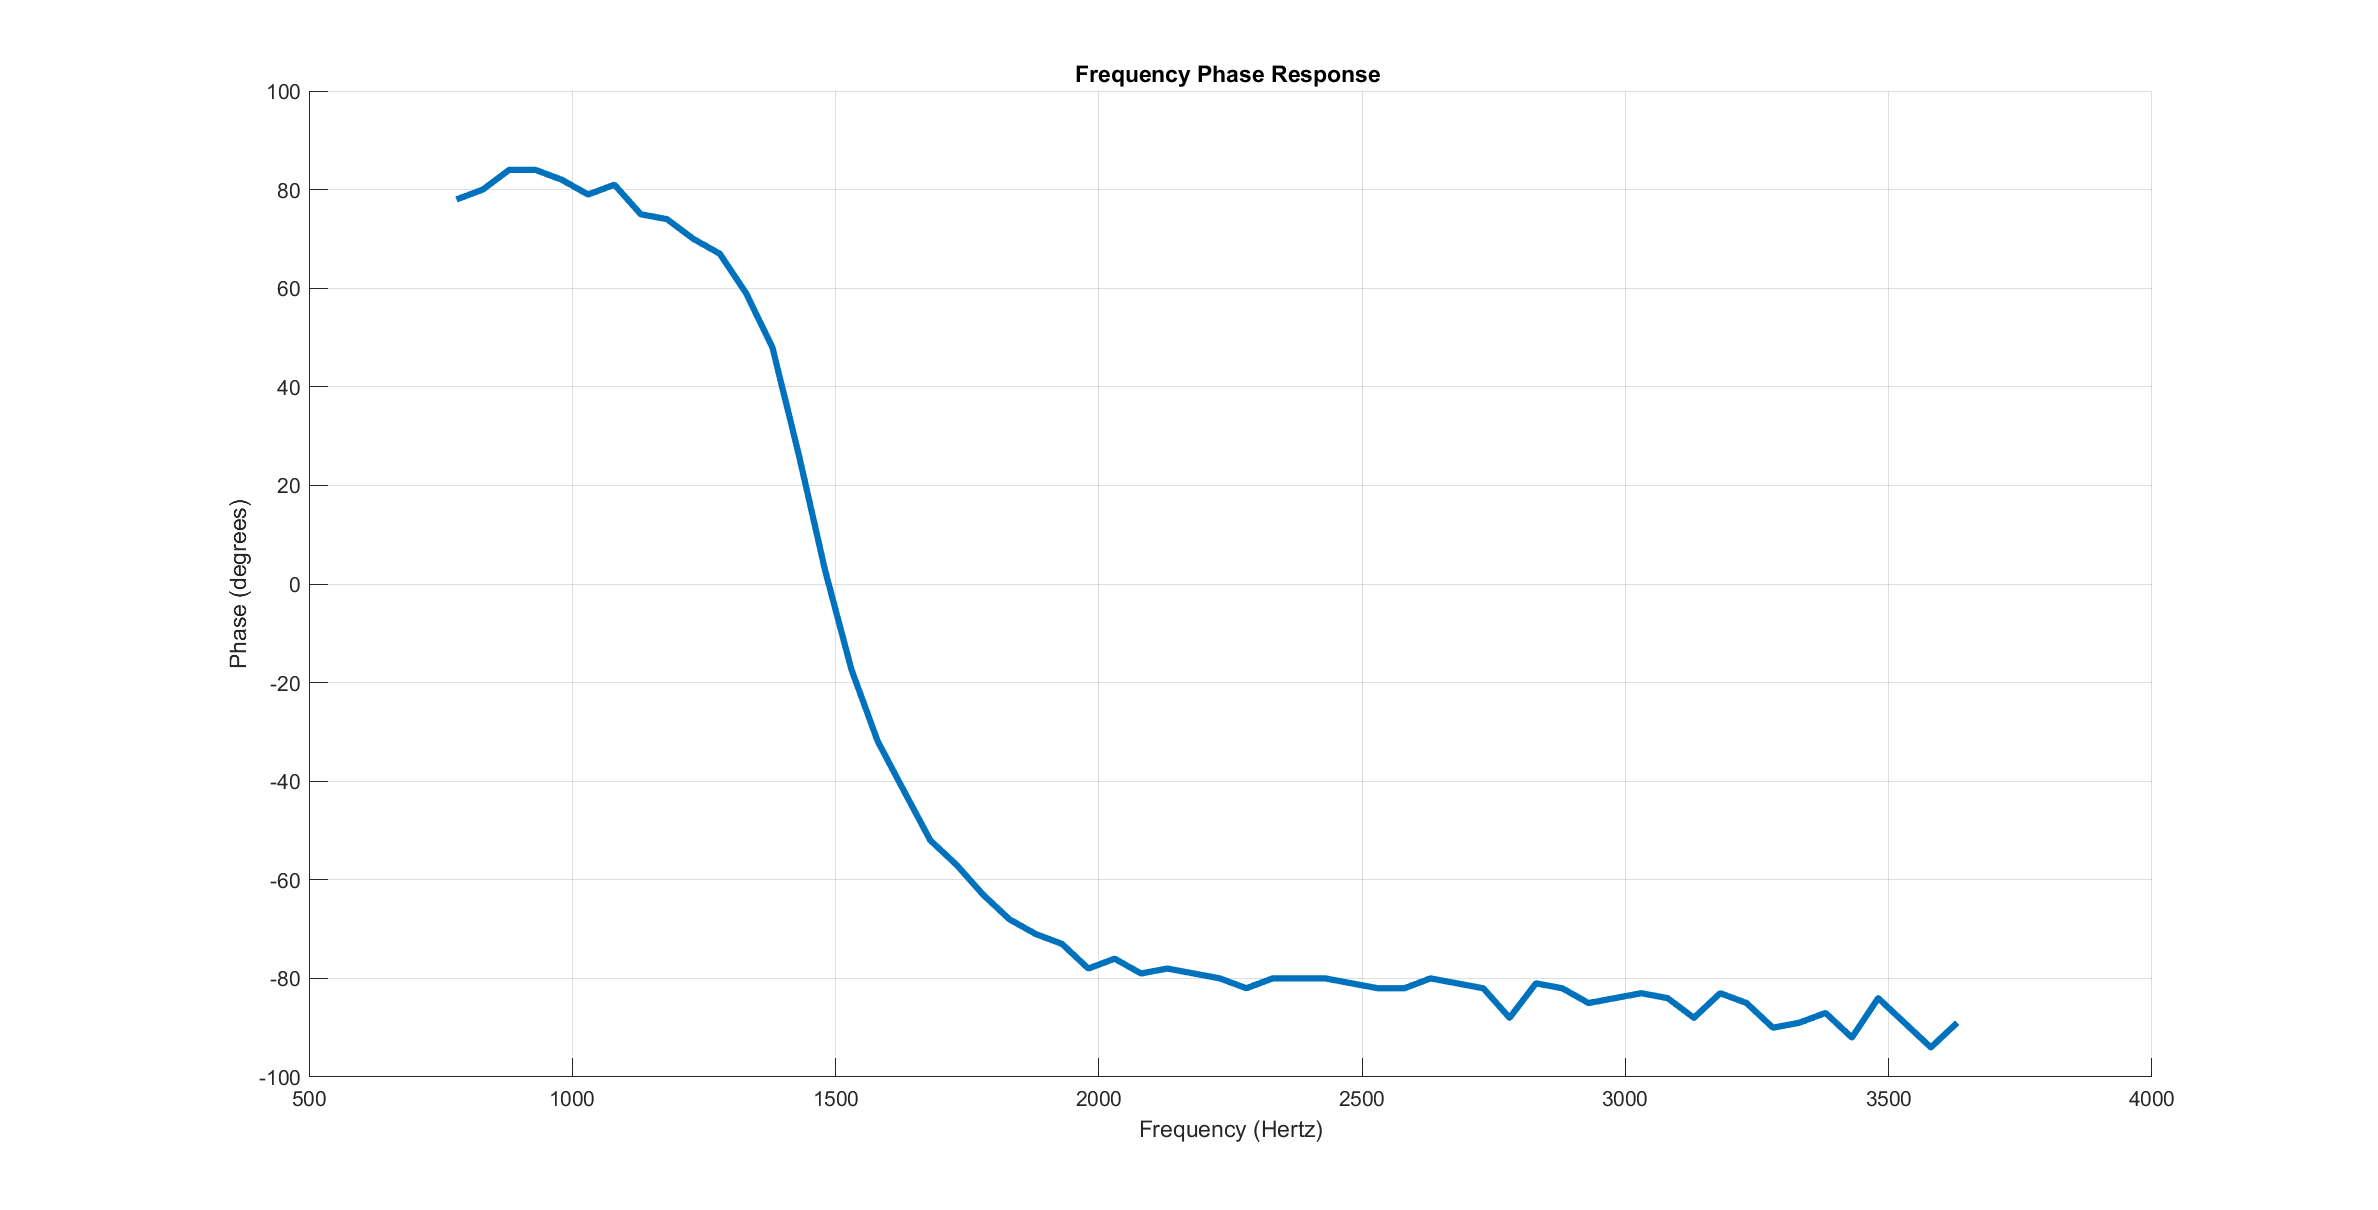
\includegraphics[width = 0.75\textwidth]{3_1_2.png}
    \caption{Phase Response of the High-Q RLC filter.}
\end{figure} 

\begin{figure}[H]
    \centering
    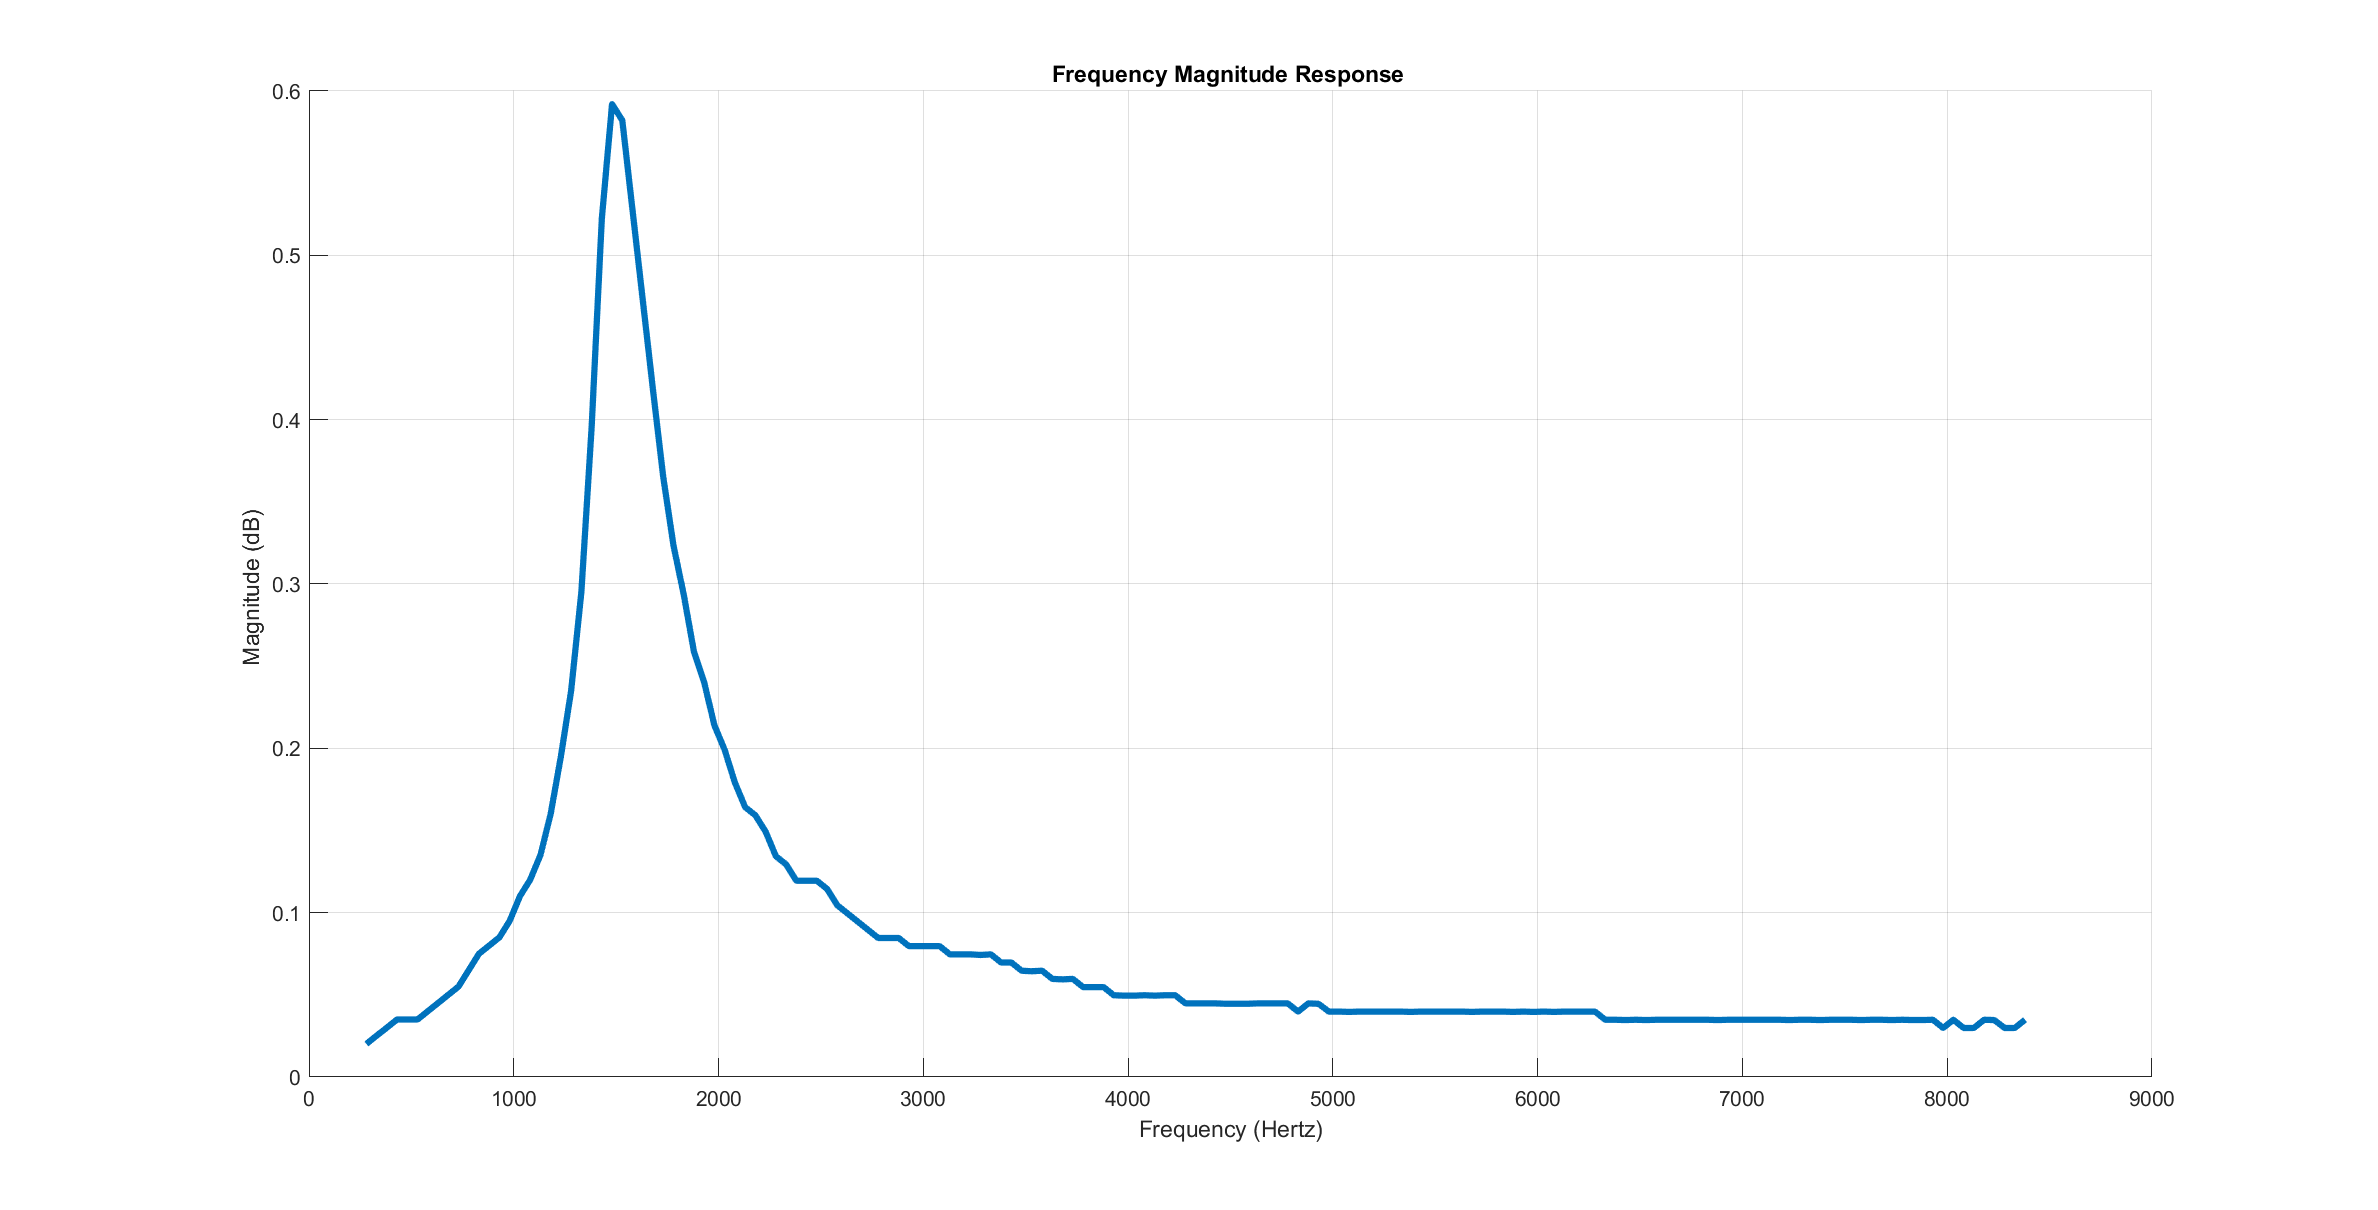
\includegraphics[width = 0.75\textwidth]{3_1_1.png}
    \caption{Magnitude Response of the High-Q RLC filter.}
\end{figure} 
The values \(\omega_{c1}\) ,\(\omega_{0}\) and \(\omega_{c2}\)  are indicated in the magnitude response plot with data pins. This filter is a bandpass filter that only allows a certain band of frequencies to pass on. The Q (Quality Factor) of the filter is calculated as 3.821, which can be considered a high Q. This also intuitively gives an idea of the sharpness of the phase angle plot.  

\subsection{Step 4}
In this step, circuit in Step 3 is used.
\subsubsection{a.}
For this step, a square wave at the resonant frequency where magnitude response is equal to 1 is applied and then input and output voltages are plotted in Figure 10.
Since this circuit passes some frequency interval to pass it is called a bandpass filter.  
\begin{figure}[H]
    \centering
    \includegraphics[width = 0.75\textwidth]{{4_1_1.png}}
    \caption{Frequency response of  square wave applied bandpass filter}
\end{figure} 
\subsubsection{b.}
For this step, circuit in Figure 11 is set and a sine wave at the resonant frequency is applied. Then, \(V_{01}\) and \(V_{02}\) plot is obtained in Figure 12.


\begin{figure}[H]
    \centering
    \includegraphics[width = 0.75\textwidth]{{STP4ct.png}}
    \caption{Circuit for step 4 part b}
\end{figure} 
\begin{figure}[H]
    \centering
    \includegraphics[width = 0.75\textwidth]{{4_2_1.png}}
    \caption{Frequency phase response of the circuit step 4 part b.}
\end{figure} 
Since there is a capacitor at the load,the capacitor discharges in the negative cycle of the input. Therefore, \(V_{01}\) is measured as a sine wave while \(V_{02}\) is 0 at the negative cycle.


\section{Conclusion}
In this experiment, Frequency Response, four different setups of filter circuits are experimented with. First, a highpass filter with a resistor and a capacitor is set, and its characteristics are observed. Then a lowpass filter with an inductor and a resistor is constructed, and its behavior is observed. A high-q RLC bandpass filter will be set, and its quality factor will be determined. Lastly, a square wave is applied to the bandpass, and a half rectified sinusoidal is filtered. As a result, the waves that are included in an oblique signal are observed.


\section*{Appendix A}
\begin{itemize}
    \item PreLab Preparation 2 hours
    \item Experimental Work 2  hours
    \item Report Writing 9 hours
\end{itemize}

\end{document}

%%%%%%%%%%%%%%%%%%%%%%   EXAMPLE TABLE   %%%%%%%%%%%%%%%%%%%%%%%%%%%%%%%%
\begin{table}[H]
\begin{center}
    \caption{Resistance reading by color code convention.}
    \vspace{2mm}
    \begin{tabular}{||c | c | c||} 
        \hline
        Color Order & Value & Tolerance \\ [0.5ex] 
        \hline\hline
        Brown / Black / Red / Gold & 1k\( \Omega \) & \( \% \) 5  \\ 
        \hline
        Yellow / Violet / Red / Gold & 4.7k\( \Omega \) & \( \% \) 5   \\
        \hline
        Brown / Grey / Orange / Gold & 18k\( \Omega \) & \( \% \) 5  \\ [1ex] 
        \hline
    \end{tabular}
\end{center}
\end{table}


%%%%%%%%%%%%%%%%%%%%%%   EXAMPLE IMAGE   %%%%%%%%%%%%%%%%%%%%%%%%%%%%%%%%
\begin{figure}[H]
\centering
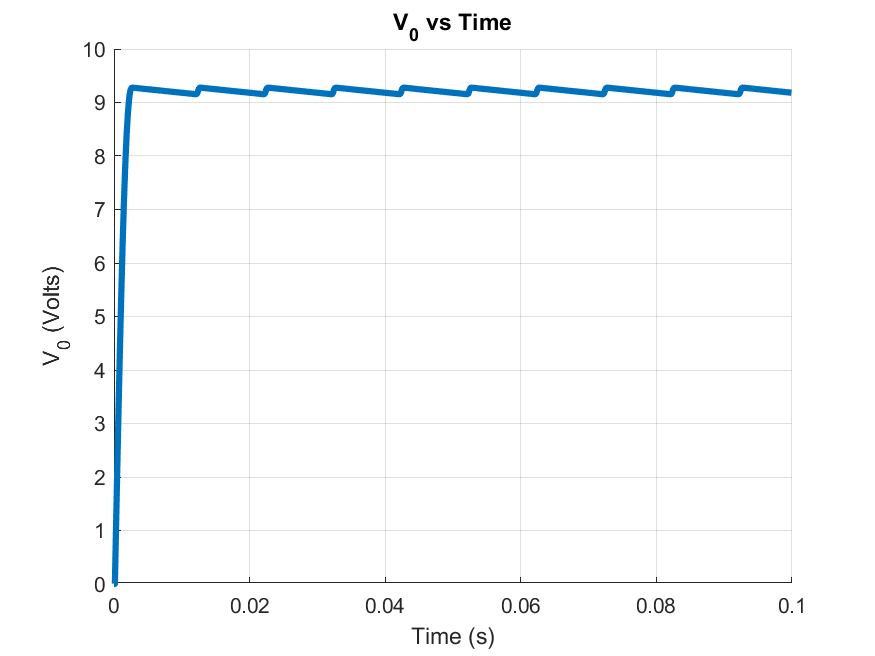
\includegraphics[width = 0.75\textwidth]{5.png}
\caption{Circuit schematic for the step 5}
\end{figure} 

%%%%%%%%%%%%%%%%%%%%%%   EXAMPLE IMAGE FROM PDF   %%%%%%%%%%%%%%%%%%%%%%%%%%%%%%%%
\begin{figure}[H] \centering{
	\includegraphics[scale=0.25]{2a_plot.pdf}}
	\caption{Experiment 2}
\end{figure}
